\documentclass[4paper,0pt]{article}
\pagestyle {plain}
\usepackage {a4wide}

\usepackage [ngerman]{babel}
\usepackage [utf8]{inputenc}
\usepackage{graphics}
\usepackage{wrapfig}

\usepackage[T1]{fontenc}

\usepackage {amsmath}
\usepackage {amsfonts}
\usepackage {amssymb}

\usepackage{graphicx}
\usepackage{pdfpages} 
\renewcommand{\familydefault}{\sfdefault}
\usepackage{helvet}
\usepackage{listings}
\usepackage{color}
\usepackage{hyperref}
\usepackage{framed}
\definecolor{shadecolor}{rgb}{0.8,0.85,1}


 \definecolor{middlegray}{rgb}{0.5,0.5,0.5}
 \definecolor{lightgray}{rgb}{0.8,0.8,0.8}
 \definecolor{orange}{rgb}{0.8,0.3,0.3}
 \definecolor{yac}{rgb}{0.6,0.6,0.1}
 
\lstset{
   basicstyle=\scriptsize\ttfamily,
   keywordstyle=\bfseries\ttfamily\color{orange},
   stringstyle=\color{blue}\ttfamily,
   commentstyle=\color{middlegray}\ttfamily,
   emph={square}, 
   emphstyle=\color{blue}\texttt,
   emph={[2]root,base},
   emphstyle={[2]\color{yac}\texttt},
   showstringspaces=false,
   flexiblecolumns=false,
   tabsize=2,
   numbers=left,
   numberstyle=\tiny,
   numberblanklines=false,
   stepnumber=0,
   numbersep=10pt,
   xleftmargin=15pt
 }

\parindent 0pt

\author{\  Alexander von Leliwa \\ Bernhard Schmitt}

\title { \huge \bf RaspberryPI Fehrnsteuerung \\  \Huge Dokumentation }

\begin{document}
\maketitle
\newpage

\tableofcontents
\newpage

\section{Beispiele}

\subsection{quellcode}

\begin{lstlisting}
#!/usr/bin/env python3
#Eine Wirkung, z.B. Pin schalten, wird ausgefuehrt

#Initialisierung

def wk_exe(art, pinnr, typ, wert):
    # art 1 --> GPIO
    if art == 1:
        import RPi.GPIO as GPIO
        GPIO.setmode(GPIO.BOARD)
\end{lstlisting}

\begin{shaded}
\begin{lstlisting}
$ ifconfig
\end{lstlisting}
\end{shaded}

\lstinputlisting
    [caption={Wlan einbinden}
       \label{lst:python},
       captionpos=t,language=Python]
{Python/datei.py}

oder mit farbe 

\begin{shaded}
\lstinputlisting
    [caption={Wlan einbinden mit farbe}
       \label{lst:python},
       captionpos=t,language=Python]
{Python/datei.py}
\end{shaded}

\subsection{links}

Auf dieser Seite befindet sich ein \hyperlink{target}{Hyperlink} auf die folgende Seite.
 
\newpage
 
Hier befindet sich das \hypertarget{target}{Ziel}. In die große, weite Welt geht 
es \href{http://de.wikipedia.org/wiki/Welt}{hier}.

\subsection{fabige frames}

\begin{shaded}bla test bla \end{shaded}

\section{Einrichten des Raspberry PI}
\subsection{Betriebssystem}

Wir verwenden das Betriebssystem \href{http://downloads.raspberrypi.org/raspbian_latest}{Raspbian} und installieren es über das Programm \href{http://downloads.raspberrypi.org/NOOBS_latestt}{NOOBS} da dieses eine einfach Erstinstallation ermöglicht. Weitere Informationen und Versionen gibt es auf dieser \href{http://www.raspberrypi.org/}{Seite} 

\subsection{WLAN-Einrichten}

Hilfreiche Links:
\href{https://www.datenreise.de/raspberry-pi-wlan-einrichten-edimax//}{Datenreise}.

\subsubsection{Stick erkennen}

Verwendet wird der \href{http://www.amazon.de/gp/product/B003MTTJOY/ref=as_li_qf_sp_asin_tl?ie=UTF8&camp=1638&creative=6742&creativeASIN=B003MTTJOY&linkCode=as2&tag=dde0b6-21}{EDIMAX Wireless Adapter}. Dieser wird nach dem einstecken vom Raspi automatisch erkannt. Testen kann man dies mit dem Befehl:

\begin{shaded}
\begin{lstlisting}
$ ifconfig
\end{lstlisting}
\end{shaded}

nun sollte auf dem Bildschirm eine Aufzählung der verschiedenen Netzwerkschnittstellen kommen. Darunter sollte auch das WLan auftauchen. 

\subsubsection{Schlafmodus deaktivieren}

Nun sollten wir den Stromsparmodus des Sticks deaktivieren. Um dies zu tun, muss eine Konfigurationsdatei für den Treiber angelegt werden:

\begin{shaded}
\begin{lstlisting}
$ sudo nano /etc/modprobe.d/8192cu.conf
\end{lstlisting}
\end{shaded}

Diese Datei bekommt folgenden Inhalt:

\begin{shaded}
\begin{lstlisting}
options 8192cu rtw_power_mgnt=0 rtw_enusbss=0
\end{lstlisting}
\end{shaded}

\subsubsection{Verbindung herstellen}

Um eine Verbindung herzustellen müssen wir eine Datei editieren:

\begin{shaded}
\begin{lstlisting}
$ sudo nano /etc/network/interfaces
\end{lstlisting}
\end{shaded}

den Inhalt wie folgt anpassen:

\begin{shaded}
\begin{lstlisting}
aus unserem Raspi kopieren
\end{lstlisting}
\end{shaded}

Abschließend muss noch die Änderung geändert werden:

\begin{shaded}
\begin{lstlisting}
$ sudo service networking restart
\end{lstlisting}
\end{shaded}

Das Programm das dieses Automatisch erledigt ist \hyperlink{target}{hier} (muss noch verlinkt werden) erklärt. 

\section{Hardware anschluss}
\section{xml Schnittstellendatei}
\section{PHP Benutzerplattform}
\section{Backend (Python Steuerung)}

Die grobe Struktur

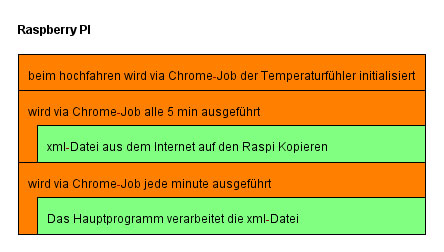
\includegraphics[width=0.8\textwidth]{Bilder/RaspberryPI.jpg}

\subsection{Chrome-Job}
\subsection{Temperaturfühler initialisieren}

Um den Temperaturfühler zu initialisieren müssen wir in der Konsole folgende Befehle eingeben:

\begin{shaded}
\begin{lstlisting}
sudo modprobe w1-gpio
sudo modprobe w1-therm
\end{lstlisting}
\end{shaded}

nun ist wurde automatisch ein Ordner angelegt welcher die Temperatur beinhaltet. er ist wie folgt zu finden:

\begin{shaded}
\begin{lstlisting}
cd /sys/bus/w1/devices/serial_number (bsp: 10-000802824e58)
\end{lstlisting}
\end{shaded}

der letzte Ordner entspricht der Serien Nummer des verwendeten Temperaturfühlers. Der Inhalt der Datei sieht in etwa so aus:

\begin{shaded}
\begin{lstlisting}
2d 00 4b ff ff 08 lO fe : crc=fe YES
2d 00 4b ff ff 08 lO fe t=22250
\end{lstlisting}
\end{shaded}

t=xxxxx gibt und hierbei die Temperatur an nur das der Wert noch durch 1000 geteilt werden muss. In diesem Beispiel haben wir also 22,250 C\\

hilfreiche links:\\

Sensor einlesen mit Datei ausgabe:
\href{http://www.gtkdb.de/index_31_2040.html}{hier}

Sensor einfaches Einlesen mit manueller Seriennummer eingabe:
\href{http://www.cl.cam.ac.uk/projects/raspberrypi/tutorials/temperature/}{hier}

\subsection{Hauptprogramm}

\begin{shaded}
\lstinputlisting
    [caption={Hauptprogramm}
       \label{lst:python},
       captionpos=t,language=Python]
{Python/Hauptprogramm.py}
\end{shaded}


\end{document}